%% main_v18_zh.tex — camera-ready 中文翻译稿（基于 main_v18.tex）
%% Compile: xelatex main_v18_zh && bibtex main_v18_zh && xelatex main_v18_zh && xelatex main_v18_zh

\documentclass{article}
\PassOptionsToPackage{numbers,sort&compress}{natbib}
\usepackage[final,main]{neurips_2026}
\usepackage[UTF8,scheme=plain,fontset=none]{ctex}
\setCJKmainfont[Path=/Library/Fonts/,AutoFakeBold=2]{Arial Unicode.ttf}
\setCJKsansfont[Path=/Library/Fonts/,AutoFakeBold=2]{Arial Unicode.ttf}
\setCJKmonofont[Path=/Library/Fonts/]{Arial Unicode.ttf}
\usepackage{amsmath,amssymb,amsthm,mathtools}
\usepackage{booktabs,multirow,array,tabularx}
\usepackage{graphicx,subcaption}
\graphicspath{{./}{../figures/}}
\usepackage{xcolor}
\usepackage[colorlinks=true,linkcolor=blue!70!black,citecolor=blue!70!black,urlcolor=blue!70!black]{hyperref}
\usepackage{algorithm,algpseudocode}
\usepackage{microtype,enumitem,xspace,nicefrac}

\newcommand{\reff}{\ensuremath{r_{\mathrm{eff}}}\xspace}
\newcommand{\SAk}{\ensuremath{\mathrm{SA}_k}\xspace}
\newcommand{\UID}{\ensuremath{\mathrm{UID}}\xspace}
\newcommand{\SSRdag}{\ensuremath{\mathrm{SSR}^{\ddagger}}\xspace}
\newcommand{\rhoSp}{\ensuremath{\rho_{\mathrm{Sp}}}\xspace}
\newtheorem{theorem}{定理}
\newtheorem{lemma}{引理}
\newtheorem{proposition}[lemma]{命题}
\newtheorem{remark}{注}
\renewenvironment{abstract}{%
  \vskip 0.075in\centerline{\large\bf 摘要}\vspace{0.5ex}\begin{quote}%
}{\par\end{quote}\vskip 1ex}

\title{跨架构迁移性受到特征宽度混淆：诊断与子空间校正}
\author{%
  Qin Liu \quad Chen Zhong \quad Fengshan ZHAO\thanks{通讯作者：Fengshan Zhao，\texttt{fs.zhao@nju.edu.cn}}\\
  南京大学新型软件技术国家重点实验室\\
  中国南京
}
\date{}

\begin{document}
\renewcommand{\figurename}{图}
\renewcommand{\tablename}{表}
\renewcommand{\refname}{参考文献}
\floatname{algorithm}{算法}
\maketitle

\begin{abstract}
在没有目标标签时选择预训练编码器，是迁移学习中的常见预处理步骤。RankMe 是一种广泛使用的无标签分数，但其验证主要局限于同一架构族。本文表明，在比较异构架构时，其有效秩会受到倒数第二层宽度的严重混淆：在各向同性随机特征模型下，RankMe 有效秩按 $\Theta(d)$ 缩放；在实验中，其跨架构排序主要追踪特征宽度，而非迁移质量。我们提出子空间校正排序（Subspace-Corrected Ranking, SCR），将目标谱信息与“同一候选编码器在目标数据和固定参考数据上的特征子空间相对几何”结合。其无超参数成员 \SSRdag 用对数有效秩减去对数子空间对齐度。在 MV、VTAB 和 EX 的 $22$ 个共同支持池--任务单元上，\SSRdag 将平均遗憾从 RankMe 的 $0.173$ 降至 $0.069$；配对差值为 $-0.1043$（按目标名称聚类的 $95\%$ 置信区间 $[-0.167,-0.040]$，$p=0.00118$）。\SSRdag 面向跨架构族选择，并非 RankMe 的通用替代品；同一架构族内部仍优先使用 RankMe。五个 MV 任务上的概念验证还表明，\SSRdag$\to$RankMe 两阶段流程可在保持相近遗憾的同时减少前向评估，但这不是一般性的成本保证。
\end{abstract}

\section{引言}
迁移学习首先要决定对目标任务微调哪个预训练编码器。当候选模型共享同一架构、仅预训练方案不同时，可以在倒数第二层特征上使用无标签分数进行低成本选择。RankMe~\citep{garrido2023rankme} 计算特征矩阵的有效秩 $\reff(H)$，并按 $\log\reff$ 排序。在其原始验证所采用的同架构场景中，候选模型的特征维度 $d$ 固定，因此宽度不会干扰排序。

实际模型库却包含 ResNet、ViT、ConvNeXt、EfficientNet 等结构完全不同的骨干网络，其倒数第二层维度相差可达一个数量级。我们发现，在这种跨架构场景中，RankMe 会系统性失败：在包含 $35$ 个架构、$132$ 个预训练变体的模型池中，它在所有任务上都选择最宽的变体，且表现差于均匀随机选择。

其机制来自近各向同性条件下 RankMe 的仅目标谱形式。修正后的 Marchenko--Pastur 推导表明，在固定正长宽比下，RankMe 有效秩按 $\Theta(d)$ 缩放，因此 $\log\reff$ 渐近等于 $\log d$ 加一个仅依赖长宽比的常数。该形式结论只针对 RankMe；“旋转不变”本身不足以推出任意分数都随 $d$ 单调变化。

我们的校正是关系式的，而非仅依赖目标谱。SCR 使用同一候选编码器分别提取目标数据和参考数据的特征，并比较二者的子空间。该分数对共同表示基变换保持不变，但并非仅由目标特征的奇异值谱决定。在完整 VTAB 支持上，$\SAk$ 与参考子空间之外的类均值方差比例高度负相关（$\rhoSp=-0.959$）。这构成机制层面的经验证据，而非下游准确率的形式保证。

\paragraph{贡献。}
（1）我们给出 RankMe 在各向同性随机特征模型下的 $\Theta(d)$ 缩放结论，并在多个异构模型池中验证严重的宽度混淆；（2）提出基于候选模型内部“目标--参考”相对几何的 SCR 及其无超参数成员 \SSRdag；（3）给出适用范围明确的两阶段流程：跨架构族用 \SSRdag，族内变体用 RankMe；（4）构建四个可复现实验池，共覆盖 $52$ 个任务单元，宽度范围为 $d\in[192,4096]$。

\section{相关工作}
RankMe~\citep{garrido2023rankme} 使用 $p_i=\sigma_i/\sum_j\sigma_j$ 定义有效秩；本文关注超出其原始同架构验证范围的异构模型池。VNE~\citep{kim2023vne} 使用归一化平方奇异值的熵，但本文不把针对 RankMe 的定理推广到 VNE。官方分类版 DiSCO~\citep{zhang2025disco} 使用目标真实标签构造类条件量，因此本文将其作为有标签比较方法，而不是零标签基线。LogME、H-score、NCTI、LEEP 等同样需要标签。子空间对齐最初用于无监督域适应~\citep{fernando2013sa}；本文则把它用于度量同一候选编码器在目标数据和固定参考数据上的通用--特定特征结构。

\section{实验设置}
\begin{table}[h]
\centering\small
\caption{四个异构评估池。宽度跨度决定混淆严重程度。}
\label{tab:pool_setup_zh}
\resizebox{\linewidth}{!}{\begin{tabular}{lccccc}
\toprule
模型池 & 架构数 & 变体数 & 任务数 & $d$ 范围 & $d_{\max}/d_{\min}$ \\
\midrule
MV（多变体） & $35$ & $119$（多变体）/$132$（全部） & $5$ & $[192,4096]$ & $21.3\times$ \\
VTAB & $24$ & $24$ & $8$ & $[192,2048]$ & $10.7\times$ \\
SSL/多模态 & $8$ & $8$ & $29$ & $[384,2048]$ & $5.3\times$ \\
EX（监督预训练） & $35$ & $51$ & $10$ & $[192,4096]$ & $21.3\times$ \\
\bottomrule
\end{tabular}}
\end{table}

有效秩严格采用 RankMe 定义：$p_i=\sigma_i/\sum_j\sigma_j$，$\reff=\exp(-\sum_i p_i\log p_i)$。对每个候选编码器 $m$，$\SAk$ 比较其目标特征与 STL-10 特征；二者由同一编码器产生，因此维度都为 $d_m$。所有主要结果使用未经额外中心化的特征矩阵，默认 $k=20$，取对数前将正值下限裁剪为 $10^{-12}$。不同候选模型的子空间从不直接比较。线性探针使用 $\ell_2$ 正则逻辑回归（$C=1$）和固定 $80/20$ 划分；策略质量以相对逐任务 oracle 的遗憾衡量。

\section{宽度混淆}
\begin{lemma}[Marchenko--Pastur 缩放]
令 $H\in\mathbb{R}^{n\times d}$ 的各行独立同分布于 $\mathcal N(0,\sigma^2I_d)$。当 $n,d\to\infty$ 且 $\gamma=n/d$ 固定时，$\reff(H)/d\to c(\gamma)>0$ 几乎处处成立，其中 $c(\gamma)$ 仅依赖长宽比。因此 $\reff(H)=\Theta(d)$。
\end{lemma}

\begin{proposition}[\SSRdag 的关系性与共同基不变性]
对候选编码器 $m$ 和 $Q\in O(d_m)$，同时将 $(H_{m,T},H_{m,R})$ 替换为 $(H_{m,T}Q,H_{m,R}Q)$，其主角、$\SAk$ 和 \SSRdag 均不变。但是，\SSRdag 并非只由 $H_{m,T}$ 的奇异值决定；它还依赖目标与参考右奇异子空间的相对几何。
\end{proposition}

RankMe 与宽度的逐任务平均 Spearman 相关在 MV、VTAB、SSL 上分别为 $0.61$、$0.879$、$0.815$；而宽度与线性探针准确率的平均相关分别为 $-0.10$、$+0.23$、$-0.45$。因此，宽度可强烈支配 RankMe，却不能可靠识别最佳迁移表示。MV 中 RankMe 在五个任务上均选择 $d=4096$ 的 VGG-16，平均遗憾 $0.319$，差于随机选择的 $0.194$；移除仅三个 VGG 变体后，RankMe 遗憾下降至 $0.144$，而 \SSRdag 在移除前后均为 $0.098$。

\begin{table}[h]
\centering\small
\caption{MV 多变体支持上的逐任务结果。}
\resizebox{\linewidth}{!}{\begin{tabular}{lrrrrlll}
\toprule
任务 & Oracle & 随机 & RankMe & \SSRdag & RankMe 选择 & \SSRdag 选择 & Oracle 架构 \\
\midrule
CIFAR-10 & .970 & .785 & .550 & .870 & vgg16 & resnet50 & convnext\_base \\
CIFAR-100 & .825 & .484 & .180 & .670 & vgg16 & resnet152 & convnext\_base \\
DTD & .740 & .564 & .445 & .720 & vgg16 & convnext\_base & convnext\_base \\
EuroSAT & .955 & .881 & .765 & .905 & vgg16 & efficientnet\_b3 & densenet201 \\
SVHN & .615 & .430 & .570 & .450 & vgg16 & efficientnet\_b3 & densenet169 \\
\bottomrule
\end{tabular}}
\end{table}

\section{子空间校正排序}
对候选编码器 $m$，令未经额外中心化的特征矩阵为 $H_{m,T}\in\mathbb R^{n_T\times d_m}$ 和 $H_{m,R}\in\mathbb R^{n_R\times d_m}$。令 $V_T,V_R\in\mathbb R^{d_m\times k_m}$ 分别包含其前导右奇异向量，其中 $k_m=\min\{k,n_T,n_R,d_m\}$，默认 $k=20$。若主角为 $\theta_1,\ldots,\theta_{k_m}$，则
\[
\SAk(H_{m,T},H_{m,R})=\frac{1}{k_m}\lVert V_T^\top V_R\rVert_F^2
=\frac{1}{k_m}\sum_{i=1}^{k_m}\cos^2\theta_i.
\]
完整流程为：使用同一候选编码器提取目标与参考特征；分别计算未经额外中心化的 SVD；保留两个前 $k_m$ 子空间；由主角计算 $\SAk$；由目标奇异值计算 RankMe 的 $\reff$；将 $\reff$ 和 $\SAk$ 裁剪到至少 $10^{-12}$；最后返回标量分数。候选模型的特征维度可以不同，因为不存在跨候选的子空间比较。

SCR 分数族定义为
\[
\mathrm{SCR}(H,T;\beta,g)=
\frac{\log\reff(H)+\beta g\bigl(\SAk(H,H_{\mathrm{ref}})\bigr)}{\log C(T)},
\]
其中 $g$ 单调递减且 $\beta\geq0$。取 $g(s)=-\log s$、$\beta=1$ 得到实际用于全部主结果的分数
\[
\boxed{\SSRdag(H,T)=\frac{\log\reff(H)-\log\SAk(H,H_{\mathrm{ref}})}{\log C(T)}}.
\]
对固定任务，正因子 $1/\log C(T)$ 不改变候选排序。该分数对共同表示基变换不变，但不是目标奇异值谱的单输入函数。

所有主实验使用 STL-10 作为实用而非理论最优的参考数据集：它规模较小、包含多类自然物体、所有候选均支持，并与七个 VTAB 目标任务不重合。我们的默认建议是选用一个通用且与目标不重叠的参考数据集。完整 $24$ 架构 VTAB 支持上，STL-10 单参考的遗憾为 $0.061$；四个预先指定参考数据集的逐目标留一中位数集成为 $0.055$。论文早期 Flowers-102 自参考结果因目标/参考泄漏而撤回。集成收益仅基于七个任务，且参考侧成本近似线性增加，因此单参考仍为默认方案。

\begin{figure}[t]
\centering
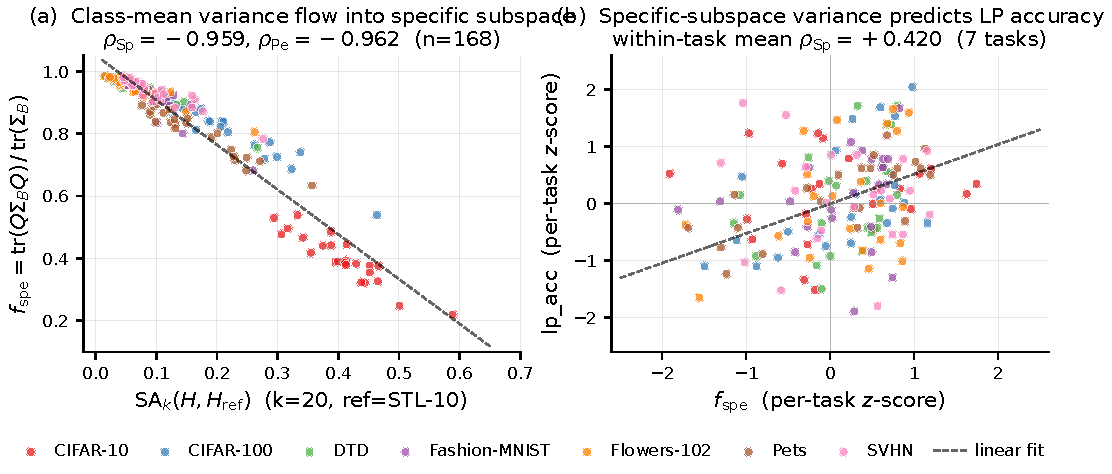
\includegraphics[width=.88\linewidth]{fig_sigma_b_flow.pdf}
\caption{（a）子空间对齐度 $\SAk$ 与架构特定子空间中的类均值方差比例 $f_{\mathrm{spe}}$ 近乎完全负相关；（b）在每个任务内部，$f_{\mathrm{spe}}$ 能预测线性探针准确率。}
\end{figure}

在 MV 的 $5$ 个任务、VTAB 的 $7$ 个非参考任务以及 EX 的 $10$ 个任务组成的 $22$ 个共同支持池--任务单元上，\SSRdag 的平均遗憾为 $0.069$，RankMe 为 $0.173$，随机选择为 $0.137$。\SSRdag 减 RankMe 的配对差值是 $-0.1043$（单元 bootstrap 的 $95\%$ CI 为 $[-0.169,-0.046]$，$p=0.00016$）。这些观测包含 $10$ 个不同目标名称，其中 $8$ 个跨模型池重复；按目标名称聚类重采样后，$95\%$ CI 为 $[-0.167,-0.040]$，双侧 $p=0.00118$（$100{,}000$ 次重采样），配对 Wilcoxon 检验为 $p=0.00254$。

\begin{table}[h]
\centering\small
\caption{$22$ 个共同支持池--任务单元上的零标签跨池比较。官方分类 DiSCO 使用目标标签，故不列入此表。}
\begin{tabular}{lrrl}
\toprule
方法 & 平均遗憾 & 标签预算 & 作用 \\
\midrule
随机选择 & $0.137$ & 零 & 参照 \\
RankMe & $0.173$ & 零 & 目标谱 \\
\textbf{\SSRdag} & $\mathbf{0.069}$ & 零 & 目标--参考几何 \\
\bottomrule
\end{tabular}
\end{table}

几何机制的验证使用完整 VTAB 支持上的 $24\times7=168$ 个架构--任务对。$\SAk$ 与参考子空间之外的类间协方差比例 $f_{\mathrm{spe}}$ 的相关为 $-0.959$；逐任务内部，$f_{\mathrm{spe}}$ 与线性探针准确率的平均相关为 $+0.420$。这只是经验机制证据，不是 \SSRdag 与下游准确率之间的理论界。

\section{两阶段与混合预算流程}
\begin{algorithm}[h]
\caption{两阶段无源模型迁移性估计流程}
\begin{algorithmic}[1]
\State \textbf{输入：}候选池 $\{(a,V_a)\}$、目标特征、参考特征。
\State \textbf{阶段 1（架构）：}对每个架构的一个规范代表计算 \SSRdag，选出架构 $a^*$。
\State \textbf{阶段 2（变体）：}对 $a^*$ 内所有变体计算 RankMe，返回最高分变体。
\end{algorithmic}
\end{algorithm}

在五个 MV 任务上，平坦策略平均评估 $118.8$ 个变体；两阶段流程平均评估 $35+3=38$ 个候选。无标签流程 \SSRdag$\to$RankMe 的遗憾为 $0.102$，接近平坦 \SSRdag 的 $0.098$，前向评估量约为其三分之一。该结果只应视为五任务概念验证，不构成一般性能或成本保证。探索性的混合预算版本在阶段 1 使用带标签 H-score：$K=5$ 时遗憾为 $0.089$，$K=35$ 时为 $0.018$。

\begin{figure}[h]
\centering
\begin{minipage}[b]{.49\linewidth}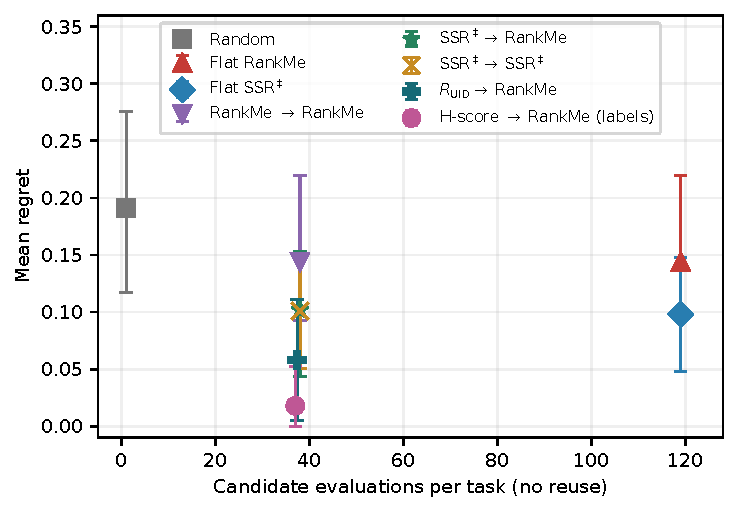
\includegraphics[width=\linewidth]{fig_pareto.pdf}\end{minipage}\hfill
\begin{minipage}[b]{.49\linewidth}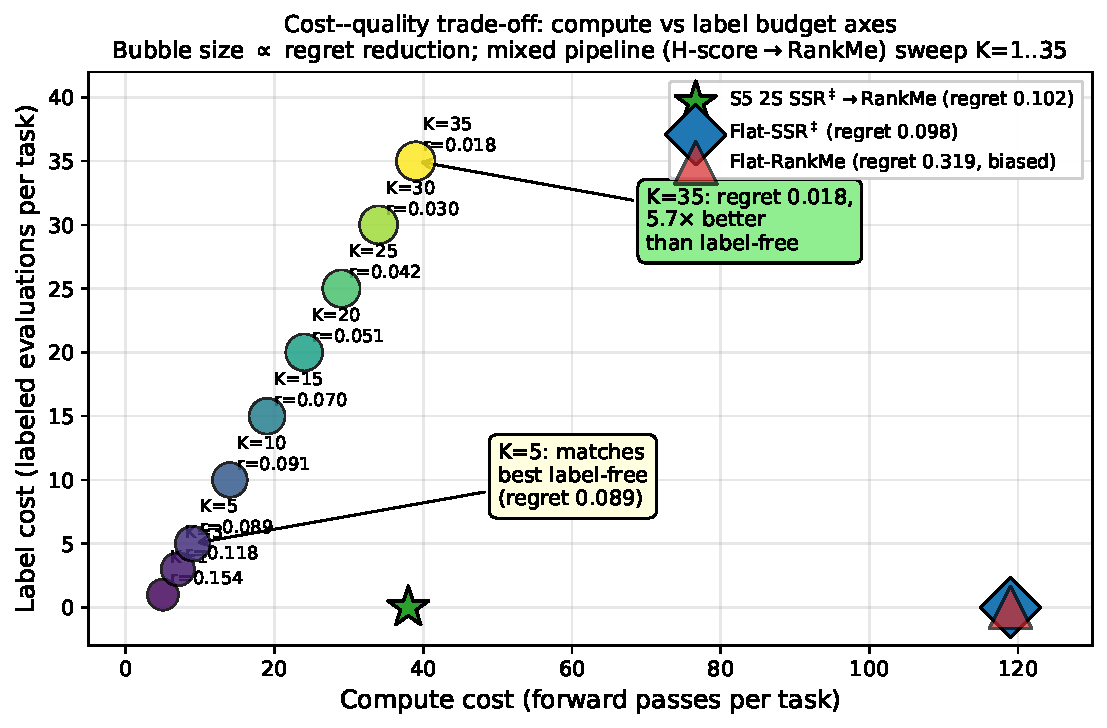
\includegraphics[width=\linewidth]{fig_costsplit.pdf}\end{minipage}
\caption{五任务 MV 概念验证。左：遗憾与前向评估次数；右：混合流程遗憾与阶段 1 标签预算 $K$。}
\end{figure}

\section{讨论与局限}
\SSRdag 适用于架构族之间的选择。当候选仅是在同一骨干上的不同预训练方案时，$\SAk$ 变化不足以追踪准确率：ViT-only 子池上 \SSRdag 相对 RankMe 的 $\Delta\rho=-0.26$（$95\%$ CI $[-0.43,-0.07]$，$p=0.010$）。因此实践规则是：跨架构族使用 \SSRdag；同族变体使用 RankMe；混合多变体模型库采用 \SSRdag 后接 RankMe。

官方 DiSCO 与 \SSRdag 的相对表现依赖模型池，尤其在 SSL 和 EX 上。更重要的是，官方分类 DiSCO 使用目标真实标签形成类条件协方差，而 \SSRdag 不使用目标标签，因此二者不能被表述为同一标签预算下的统一优劣关系。

\begin{table}[h]
\centering\small
\caption{各模型池上的官方 PCA-128 分类 DiSCO。$G$ 为连续、近等大小的谱分组数。}
\begin{tabular}{lrrr}
\toprule
模型池 & 任务数 & $G=6$ 遗憾 & $G=8$ 遗憾 \\
\midrule
MV & $5$ & $0.146$ & $0.146$ \\
VTAB（排除 STL-10） & $7$ & $0.067$ & $0.040$ \\
EX & $10$ & $0.045$ & $0.049$ \\
SSL & $29$ & $0.045$ & $0.042$ \\
\bottomrule
\end{tabular}
\end{table}

本研究仍有四项主要局限：参考数据集选择是启发式的；子空间对齐与下游准确率之间没有形式保证；相对有标签方法的性能依赖模型池；两阶段实验仅有五个 MV 任务。本文的严格主张仅是：在所评估的异构共同支持上，\SSRdag 校正了 RankMe 的跨架构族宽度混淆。

\section{结论}
在异构架构池中，RankMe 会受到特征宽度的严重混淆：在给定各向同性模型下，其有效秩按 $\Theta(d)$ 缩放，因此可能按宽度而非迁移质量排序。\SSRdag 使用同一候选编码器内部的目标--参考子空间关系，补充目标谱所缺少的信息。在 $22$ 个完整共同支持单元上，它将平均遗憾从 $0.173$ 降至 $0.069$（差值 $-0.1043$；目标聚类 $95\%$ CI $[-0.167,-0.040]$，$p=0.00118$）。结果支持跨架构族零标签选择使用 \SSRdag、同架构族选择使用 RankMe，同时把参考设计、下游保证、模型池依赖性和更广泛的两阶段验证留作未来工作。

\section*{致谢}

本工作得到“111 中心”（编号 B26023）和教育部基础学科与交叉学科突破计划（编号 JYB2025XDXM118）的支持。

\appendix
\section{Marchenko--Pastur 推导}
\begin{proof}[引理证明]
写作 $\reff(H)=\exp(H_{\mathrm{ent}}(\mathbf p))$，其中 RankMe 使用 $p_i=\sigma_i/\sum_j\sigma_j$。令 $\lambda_i=\sigma_i^2/(n\sigma^2)$，经验测度包含全部 $d$ 个特征值，包括 $d>n$ 时的零特征值。由 Marchenko--Pastur 定律~\citep{marchenko1967distribution}，该测度几乎处处收敛到 $\mu_\gamma$。定义
$S_d=d^{-1}\sum_j\sqrt{\lambda_j}$ 与 $m_{1/2}=\int\sqrt{x}\,\mathrm d\mu_\gamma(x)$。公共尺度 $\sigma\sqrt n$ 在 RankMe 中抵消，并有有限维恒等式
\[
H_{\mathrm{ent}}(\mathbf p)=\log d+\log S_d-
\frac{1}{2S_d}\frac1d\sum_i\sqrt{\lambda_i}\log\lambda_i.
\]
因此，取 $0\log0=0$，MP 极限给出
\[
H_{\mathrm{ent}}(\mathbf p)=\log d+\log m_{1/2}-
\frac{1}{2m_{1/2}}\int\sqrt{x}\log x\,\mathrm d\mu_\gamma(x)+o(1).
\]
对任意固定正长宽比，上述矩均有限，包括谱支撑到达零或在零点存在原子的情形。因此 $\reff(H)/d\to c(\gamma)>0$，即 $\reff(H)=\Theta(d)$。
\end{proof}

VTAB 上可获得诊断的架构--任务对中，类协方差统计量 $\eta_\Sigma$ 的中位数为 $0.022$、均值为 $0.035$，且 $93.3\%$ 小于 $0.1$。这说明各向同性近似与这些表示具有经验相关性，但不是对 RankMe 排序的界，也不是其他旋转不变分数的定理。

\begin{figure}[h]
\centering
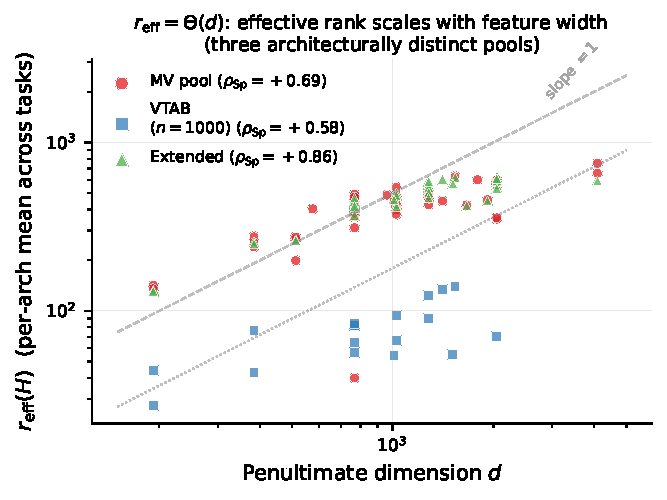
\includegraphics[width=.62\linewidth]{fig_reff_d_scatter.pdf}
\caption{各架构跨任务平均后的有效秩与倒数第二层维度（双对数坐标）。三种模型池均呈正向秩相关；斜率为 1 的虚线仅作视觉参考。}
\end{figure}

\section{各模型池与消融补充}
\paragraph{MV。}库存含 $132$ 个 ImageNet-1k 预训练变体；架构选择和两阶段比较使用属于至少含两个变体的 $35$ 个架构族的固定 $119$ 变体支持。特征宽度从 ViT/DeiT-tiny 的 $192$ 到 VGG-16 的 $4096$。仅保留 CNN 的 $78$ 个变体后，RankMe 与宽度的相关仍为 $+0.57$，因此混淆并非 ViT/CNN 差异造成。

\paragraph{SSL/多模态。}该池含 $8$ 个编码器和 $29$ 个任务，宽度为 $384$--$2048$。RankMe 在 $25/29$ 个任务上选择宽度为 $2048$ 的 ResNet 类编码器，平均遗憾 $0.103$，随机为 $0.066$。官方 PCA-128 DiSCO 的 $G=6/8$ 遗憾为 $0.045/0.042$；旧代理实现的 $0.026$ 被撤回，完整特征官方实现为 $0.057/0.047$。早期回复草稿中的 $0.077/0.071$ 不对应任何保留输出，属于转录错误。

\paragraph{VTAB。}最终模型池包含在全部八个数据集上同时具备特征和线性探针值的 $24$ 个架构。ResNet-152 仅有一个数据集的特征，因此统一排除。STL-10 仅作参考，并从共同支持目标中排除。$k=20$ 时单参考遗憾为 $0.061$，目标不重叠的留一集成为 $0.055$；早期消融显示 $k\in[10,50]$ 较稳定。

\paragraph{EX。}EX 含 $51$ 个监督预训练变体、$35$ 个规范架构和 $10$ 个任务。\SSRdag 遗憾为 $0.060$，RankMe 为 $0.144$；使用目标标签的官方 DiSCO 在 $G=6/8$ 时为 $0.045/0.049$。

\paragraph{负结果。}加入 TwoNN 内在维度并未改善排序：MV 多变体支持上的平均 $\Delta\rho=-0.538$（$95\%$ CI $[-0.782,-0.270]$）。在 $-\alpha\log\SAk$ 族内，$\alpha\in[0.5,2]$ 的遗憾为 $0.093$--$0.162$；方向反转控制 $-\log(1-\SAk)$ 的遗憾为 $0.366$，说明校正方向很重要。我们采用无需调参的 $\alpha=1$。

\bibliographystyle{plainnat}
\bibliography{references}

\end{document}
